% Document information
\newcommand{\titleinfo}{Zusammenfassung ProgCpp}
\newcommand{\authorinfo}{Sandro Pedrett}
\newcommand{\version}{1.0}
\newcommand{\versioninfo}{FS21}
% Header
\include{Template/Header}

% Setup Source Code
\lstset{ 
	backgroundcolor=\color{white},   % choose the background color; you must add \usepackage{color} or \usepackage{xcolor}; should come as last argument
	basicstyle=\footnotesize,        % the size of the fonts that are used for the code
	breakatwhitespace=true,         % sets if automatic breaks should only happen at whitespace
	breaklines=true,                 % sets automatic line breaking
	captionpos=b,                    % sets the caption-position to bottom
	commentstyle=\color{ForestGreen},    % comment style
	escapeinside={\%*}{*)},          % if you want to add LaTeX within your code
	extendedchars=true,              % lets you use non-ASCII characters; for 8-bits encodings only, does not work with UTF-8
	frame=single,	                   % adds a frame around the code
	keepspaces=true,                 % keeps spaces in text, useful for keeping indentation of code (possibly needs columns=flexible)
	language=C++,                      % the language of the code
	numbersep=5pt,                   % how far the line-numbers are from the code
	rulecolor=\color{black},         % if not set, the frame-color may be changed on line-breaks within not-black text (e.g. comments (green here))
	showspaces=false,                % show spaces everywhere adding particular underscores; it overrides 'showstringspaces'
	showstringspaces=false,          % underline spaces within strings only
	showtabs=false,                  % show tabs within strings adding particular underscores
	stepnumber=2,                    % the step between two line-numbers. If it's 1, each line will be numbered
	tabsize=2,	                   % sets default tabsize to 2 spaces
	title=\lstname,                   % show the filename of files included with \lstinputlisting; also try caption instead of title
	stringstyle=\ttfamily\color{red!50!brown},
	keywordstyle=\color{blue}\bfseries,
}

% Document
\begin{document}

\input{Sections/Einführung}
\section{OOP}

\subsection{Klassendiagram}
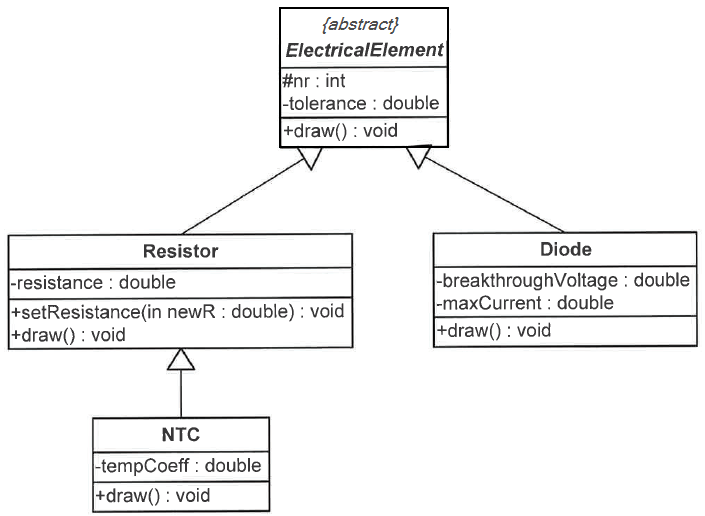
\includegraphics[width=\columnwidth]{Images/classdiagram}
\newpage

\subsection{VTable}
\lstinputlisting{Examples/Drink.h}

\includegraphics[width=\columnwidth]{Images/vtable}



\newpage
\section{C++ Features}

\subsection{Std-Library}
\begin{tabular}{ll}
\textit{$<$\textbf{iomanip}$>$} & iostream manipulators \\
\textit{$<$\textbf{iostream}$>$} & Basic stream I/O functionality \\
\textit{$<$iterator$>$} & Class for traversing a sequence \\
\textit{$<$limits$>$} & Properties of numeric types \\
\textit{$<$list$>$} & Ordered sequences \\
\textit{$<$map$>$} & Associative containers with key/value pairs \\
\textit{$<$\textbf{stdexcept}$>$} & Additional standard exception classes \\
\textit{$<$\textbf{cassert}$>$} & Compile assertions \\
\textit{$<$\textbf{string}$>$} & Sequences of characters \\
\textit{$<$typeinfo$>$} & Run-time type identification \\
\textit{$<$cstddef$>$} & Default types NULL, size\_t etc  \\
\end{tabular}


\subsection{I/O}
\lstinputlisting{Examples/io.h}

\subsection{Formatting}
\begin{tabular}{l|p{7cm}}
	\textbf{Flag} & \textbf{Wirkung} \\
	\toprule
	boolalpha & bool‐Werte werden textuell ausgegeben \\ \hline
	dec & Ausgabe erfolgt dezimal \\\hline
	fixed & Gleitkommazahlen im Fixpunktformat \\\hline
	\textbf{hex} & Ausgabe erfolgt hexadezimal \\\hline
	internal & Ausgabe innerhalb Feld \\\hline
	left & linksbündig \\\hline
	oct & Ausgabe erfolgt oktal \\\hline
	right & rechtsbündig \\\hline
	scientific & Gleitkommazahl wissenschaftlich (Mantisse und Exponent) \\\hline
	\textbf{showbase} & Zahlenbasis wird gezeigt \\\hline
	showpoint & Dezimalpunkt wird immer ausgegeben \\\hline
	showpos & Vorzeichen bei positiven Zahlen anzeigen \\\hline
	skipws & Führende Whitespaces nicht anzeigen \\\hline
	unitbuf & Leert Buffer des Outputstreams nach Schreiben \\\hline
	uppercase & Alle Kleinbuchstaben in Grossbuchstaben wandeln\\\hline
	setprecision & Definiert Nachkommastellen
\end{tabular}\\
~\\ 
\noindent\textbf{Beispiel:}\\
\begin{lstlisting}
	cout << showbase << hex << 27; // Ausgabe: 0x1b
\end{lstlisting}

\subsection{Operator Overloading}
Folgende Operatoren können überschrieben werden:\\
new delete new[] delete[] $+\quad$ $-\quad$ $*\quad$ $/\quad$ $\%\quad$ $\verb|^|\quad$ $\&\quad$ $|\quad$ $~\quad$ $!\quad$ $=\quad$ $<\quad$ $>\quad$ $+=\quad$ $-=\quad$ $*=\quad$ $/=\quad$ $\%=\quad$ $^=\quad$ $\&=\quad$ $|=\quad$ $<<\quad$ $>>\quad$ $>>=\quad$ $<<=\quad$ $==\quad$ $!=\quad$ $<=\quad$ $>=\quad$ $\&\&\quad$ $||\quad$ $++\quad$ $--\quad$ $,\quad$ $->*\quad$ $->\quad$ $( )\quad$ $[ ]$
~\\ ~\\
In dieser Tabelle steht $@$ als Platzhalter für alle Operatoren.\\ ~\\
\begin{tabular}{l|l|l}
	\textbf{Expression} & \textbf{as Member} & \textbf{As non-member} (friend) \\
	\toprule
	@a & (a).operator@() & operator@(a) \\
	a@b & (a).operator@(b) & operator@(a,b) \\
	a=b & (a).operator=(b) & - \\
	a(b) & (a).operator()(b) & - \\
	a[b] & (a).operator[](b) & - \\
	a-$>$b & (a).operator-$>$(b) & - \\
\end{tabular}
~\\ ~\\
\noindent
= [] () und $->$ müssen als Elementfunktion (nicht mit friend) implementiert werden. Alle anderen Operatoren werden typischerweise mit friend in der Klasse definiert.\\~\\

\lstinputlisting{Examples/Resistor.h}
\lstinputlisting{Examples/Resistor.cpp}


\noindent\textbf{Friend} wird oft für Operator Overloading verwendet, um Zugriff auf die lokalen Variablen der Klasse zu erhalten. Siehe auch non-member declaration\\ ~\\

\noindent\textbf{Implizit-Cast} können auch gleich wie Operator Overloading verwendet werden.
\begin{lstlisting}
struct X {
  //implicit. int n = x; oder int n = static_cast<int>(x);
  operator int() const { return 7; }
		
  // explicit. nur int* n = static_cast<int*>(x);
  explicit operator int*() const { return nullptr; }
};
\end{lstlisting}

\newpage
\subsection{Templates}
Templates sind für Bibliotheken gut geeignet, da sie nur Code erzeugen, wenn diese auch benutzt werden. Vorsicht bei inline templates Funktionen, diese können Code aufblähen.
\lstinputlisting{Examples/Stack.h}
\newpage
\subsection{Exception}
Fehler sind Abweichungen zur Spezifikation, Exception sind abnormale Bedingungen bei der Programmausführung. Im Unterschied zu anderen Programmiersprachen, kann c++ alle Typen werfen. zB könnten Literals oder Ints geworfen werden.

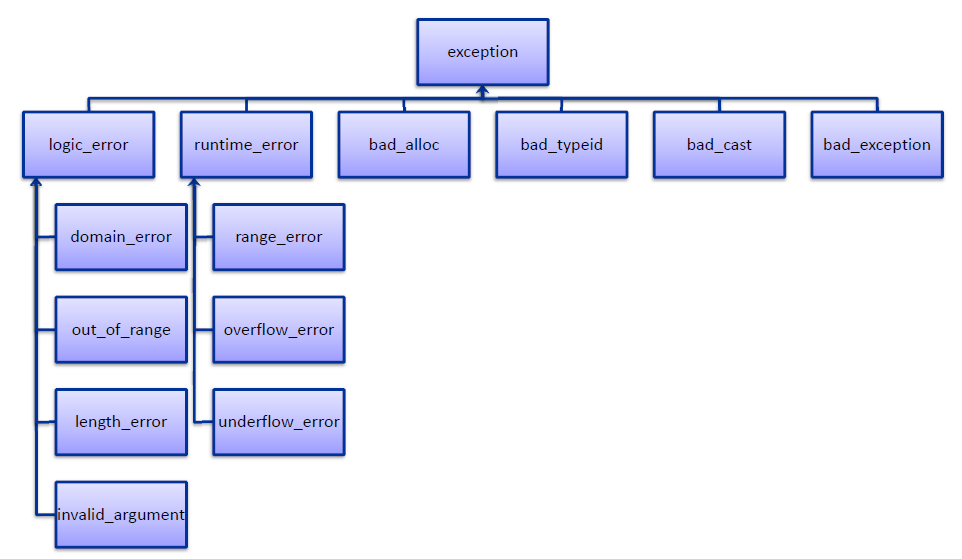
\includegraphics[width=\columnwidth]{Images/exceptions}


\noindent \textbf{WICHTIG}: Der allgemeinste Handler muss immer der letzte catch-Handler sein!
\lstinputlisting{Examples/StackException.h}

\subsection{Asserts}
\lstinputlisting{Examples/asserts.h}

\noindent \textbf{Output}:\\
\textcolor{red}{test: ../src/asserts.h:6: int main(): Assertion `a $<$ 5' failed.}\\
~\\
Schema: [Filename]:[ColNr]: [Function Signature]: Assertion '[condition]' failed







\end{document}